\documentclass[b5paper, 10 pt, twoside]{book}

%\usepackage[a4,frame,axes,cross,pdftex,center]{crop}
\usepackage[dvipsnames]{xcolor}
\usepackage[utf8]{inputenc}
\usepackage[english]{babel}
\usepackage{amsmath}
\usepackage[T1]{fontenc}
\usepackage{multicol}
\usepackage{mathtools}
\usepackage{float}
\usepackage{amssymb}
\usepackage{xfrac}
\usepackage{hhline}
\usepackage{doi}
\usepackage{amsthm} 
\usepackage{ytableau}
\usepackage{braket}
\usepackage{csquotes}
\usepackage{titling}
\newcommand{\be}{\begin{equation}}
\newcommand{\ee}{\end{equation}}
\renewcommand{\thempfootnote}{\arabic{mpfootnote}}
\setlength{\droptitle}{-3cm}
\usepackage{caption}
\usepackage{graphicx}
\usepackage{subfiles}
\usepackage[makeroom]{cancel}
\usepackage{tensor}
\usepackage{youngtab}

\usepackage[most]{tcolorbox}

\newtcolorbox{myalertbox}[1]{
  enhanced,
  colback=gray!10,
  colframe=gray!70!black,
  boxrule=0.5mm,
  arc=3mm,
  breakable,
  title=#1
}



\numberwithin{equation}{section}
\newtheorem{cor}{Corollary}[section]
\newtheorem{theo}{Theorem}[section]
\newtheorem{prop}{Proposition}[section]
\newtheorem{defi}{Definition}[section]
\newtheorem{assu}{Assumption}[section]
\newtheorem{rem}{Remark}[section]
\newtheorem{lemma}{Lemma}[section]
\newcommand{\eps}{\varepsilon} 
\usepackage[utf8]{inputenc}
\usepackage[T1]{fontenc}
\usepackage{xspace,
	amsthm,
	amsmath,
	amssymb,
	bbm,
	%showkeys,
	%refcheck
	tikz,
	graphicx,
	keyval,
       xcolor}
\usepackage{float}
\usepackage{subfig}

\DeclareGraphicsExtensions{.png, .pdf}
\DeclareMathOperator\arctanh{arctanh}
\usepackage{algorithm}
\usepackage{algpseudocode}
\usepackage{hyperref}
\usepackage{caption}
\usepackage{url}

\captionsetup{font={footnotesize},format=hang,justification=raggedright,labelfont={bf},margin={1.2cm,0cm}}
%\captionsetup[wrapfigure]{font={footnotesize},indention=-0.5cm,labelfont={bf}}
%,width=.85\textwidth
%indention=.5cm
\usepackage{multicol} % This is so we can have multiple columns of text side-by-side
%\columnsep=100pt % This is the amount of white space between the columns in the poster
%\columnseprule=3pt % This is the thickness of the black line between the columns in the poster

\usepackage[top=3cm,bottom=3cm,right=2cm,left=2.5cm]{geometry}
%\usepackage{geometry}
%\geometry{hmargin={3.5cm,3.5cm}}
%\geometry{vmargin={5cm,3cm}}

\usepackage[hyperref=true,
            url=false,
            isbn=false,
            backref=false,
            style=custom-numeric-comp,
            citereset=chapter,
            refsection=chapter,
            maxcitenames=3,
            maxbibnames=100,
            backend=biber,refsection=chapter,defernumbers=true,
            block=none]{biblatex}


\defbibheading{bibbysubsect}{\section*{References for Chapter \ref{blx:refsection\therefsection}}}
\bibliography{references}
\def\urlprefix{}\def\href#1#2#3#4{\ifstrequal{#2}{[link]}{}{#2\newline}}
\usepackage{fancyhdr}
%\pagestyle{fancy}
%
%\fancyhf{}
%\pagestyle{fancy}
%\renewcommand{\chaptermark}[1]{\markboth{\thechapter.\ #1}{}}
%\renewcommand{\sectionmark}[1]{\markright{\thesection\ #1}}
%\fancyhf{}
%\fancyhead[LE,RO]{\thepage}
%\fancyhead[CE]{\nouppercase{\leftmark}}
%\fancyhead[CO]{\nouppercase{\rightmark}}

%%%%%%%%%%%%%%%%%%%%%%%%%%%%%%%%%%%%%%%%%%%%%%%%%%%%%%%%%%%%%%%%%%%%%%%%%%%%%%%%%%%%%
%%%%%%%%%%%%%%%%%%%%%%%%%%%%%%%%%% DISEGNI %%%%%%%%%%%%%%%%%%%%%%%%%%%%%%%%%%%%%%%%%%
%%%%%%%%%%%%%%%%%%%%%%%%%%%%%%%%%%%%%%%%%%%%%%%%%%%%%%%%%%%%%%%%%%%%%%%%%%%%%%%%%%%%%

\tikzstyle{nodino}=[circle,draw,fill,inner sep=0pt,minimum size=0.5mm]
\tikzstyle{infinito}=[circle,inner sep=0pt,minimum size=0mm]
\tikzstyle{nodo}=[circle,draw,fill,inner sep=0pt, minimum size=0.5*width("k")]
\tikzstyle{nodo_vuoto}=[circle,draw,inner sep=0pt, minimum size=0.5*width("k")]
\usetikzlibrary{graphs}
\tikzset{every loop/.style={min distance=10mm,in=300,out=240,looseness=10}}
\tikzset{place/.style={circle,thick,draw=blue!75,fill=blue!20,minimum
		size=6mm}}
\tikzset{place2/.style={circle,thick,draw=red!75,fill=red!20,minimum
		size=6mm}}
\pdfsuppresswarningpagegroup=1
\usepackage{xcolor}

\definecolor{DEblue}{rgb}{0.08,0.24,0.54}
\definecolor{DEgreen}{rgb}{0.07,0.76,0.75}
\definecolor{DEorange}{rgb}{0.92,0.50,0.04}		

%%%%%%%%%%%%%%%%%%%%%%%%%%%%%%%%%%%%%%%%%%%%%%%%%%%%%%%%%%%%%%%%%%%%%%%%%%%%%%%%%%%%%
%%%%%%%%%%%%%%%%%%%%%%%%%%%%%%%%%% COMANDI %%%%%%%%%%%%%%%%%%%%%%%%%%%%%%%%%%%%%%%%%%
%%%%%%%%%%%%%%%%%%%%%%%%%%%%%%%%%%%%%%%%%%%%%%%%%%%%%%%%%%%%%%%%%%%%%%%%%%%%%%%%%%%%%

\newcommand{\f}{\frac}

\newcommand{\G}{{\mathcal{G}}}
\newcommand{\I}{{\mathcal{I}}}
\newcommand{\dip}{\eta^{dip}}
\newcommand{\ut}{u_{T}}
%\newcommand{\util}{u_{\widetilde{T}}
\newcommand{\Htau}{H_\tau^1}
\newcommand{\Htaumu}{H_{\tau,\mu}^1(\mathbb{R})}
\newcommand{\HtauFT}{H_{\tau,FT}^1(\mathbb{R})}
\newcommand{\unorm}{\|u\|_{L^2(\mathbb{R})}}
\newcommand{\udot}{\|u'\|_{L^2(\mathcal{G})}}
\newcommand{\udotr}{\|u'\|_{L^2(\mathbb{R})}}
\newcommand{\udotrneg}{\|u'\|_{L^2(\mathbb{R_-})}}
\newcommand{\udotrpos}{\|u'\|_{L^2(\mathbb{R_+})}}
\newcommand{\uLp}{\|u\|_{L^p(\mathcal{G})}}
\newcommand{\uLpr}{\|u\|_{L^p(\mathbb{R})}}
\newcommand{\uLtwor}{\|u\|_{L^2(\mathbb{R})}}
\newcommand{\uLtwo}{\|u\|_{L^2(\mathcal{G})}}
\newcommand{\HmuG}{H_\mu^1(\mathcal{G})}
\newcommand{\HmuR}{H_\mu^1(\rr)}
\newcommand{\uLsix}{\|u\|_{L^6(\mathcal{G})}}
\newcommand{\uHone}{\|u\|_{H^1(\G)}}
\newcommand{\uLsixcompact}{\|u\|_{6,\K}}
\newcommand{\K}{\mathcal{K}}
\newcommand{\h}{\mathcal{H}}
\newcommand{\om}{\omega}
\newcommand{\V}{\mathcal{V}}
\newcommand{\F}{{\mathcal{F}}}
\newcommand{\Q}{{\mathcal{Q}}}
\newcommand{\B}{{\sum\limits_{k=1}^{n}\sum\limits_{j=n+1}^{n+m} \alpha_{k,j}}}
\newcommand{\A}{\mathcal{A}_\alpha}
\newcommand{\J}{{\mathcal{J}}}
\newcommand{\D}{{\mathcal{D}}}

%\newcommand*\E{\`E\xspace}
\newcommand{\overbar}[1]{\mkern1.3mu\overline{\mkern-1.3mu#1\mkern-1.3mu}\mkern 1.3mu}
\newcommand{\EEK}{\mathcal{E}_\G(m,\K)}
\newcommand{\elevel}{\mathcal E}


% removes period at the very end of bibliographic record
\renewcommand{\finentrypunct}{}

% removes period after DOI and suppresses capitalization
% of the word following DOI ("See p. xx" -> "see p. xx")
\renewcommand{\newunitpunct}{\addspace\midsentence}

\DeclareFieldFormat{journaltitle}{\mkbibemph{#1},} % italic journal title with comma
\DeclareFieldFormat[inbook,thesis]{title}{\mkbibemph{#1}\addperiod} % italic title with period
\DeclareFieldFormat[article]{title}{#1} % title of journal article is printed as normal text
\DeclareFieldFormat[article]{volume}{\textbf{#1}\addcolon\space} % makes volume of journal bold and adds colon
\DeclareFieldFormat{pages}{#1} % removes pagination (p./pp.) before page numbers

\newlength{\spc}
\newcommand{\sjcitep}[2][]{% new command with two arguments: optional (#1) and mandatory (#2)
        \settowidth{\spc}{#1}% set value of \spc variable to the width of #1 argument
        \addtolength{\spc}{-1.8\spc}% subtract from \spc about two (1.8) of its values making its magnitude negative
        #1% print the optional argument
        \hspace*{\spc}% print an additional negative spacing stored in \spc after #1
        \supershortnotecite{#2}}% print (cite) the mandatory argument

\newcommand\vv{\textsc{v}}

\newcommand{\dx}{\,dx}
\newcommand{\dy}{\,dy}
\newcommand{\dt}{\,dt}
\newcommand{\ds}{\,ds}
\newcommand{\intX}{\int_{X_{j,k}}|u'(t)|\,dt}
\newcommand{\intY}{\int_{Y_{i,k}}|u'(t)|\,dt}
\newcommand{\intZ}{\int_{Z_{i,j}}|u'(t)|\,dt}
\newcommand{\intRneg}{\int_{-\infty}^{0}}
\newcommand{\intRpos}{\int_{0}^{+\infty}}
\newcommand{\intxneg}{\int_{-\infty}^{x_-}}
\newcommand{\intxpos}{\int_{x_+}^{+\infty}}
\newcommand{\intone}{\int_{-1}^{1}}
\newcommand{\intTtilde}{\int_{\widetilde{T}_-}^{\widetilde{T}_+}}
\newcommand{\intT}{\int_{T_-}^{T_+}}

%%%%%%%%%%%%%%%%%%%%%%%%%%%%%%%%%%%%%%%%%%%%%%%%%%%%%%%%%%%%%%%%%%%%%%%%%%%%%%%%%%%%%
%%%%%%%%%%%%%%%%%%%%%%%%%%%%%%%%%% TEOREMI %%%%%%%%%%%%%%%%%%%%%%%%%%%%%%%%%%%%%%%%%%
%%%%%%%%%%%%%%%%%%%%%%%%%%%%%%%%%%%%%%%%%%%%%%%%%%%%%%%%%%%%%%%%%%%%%%%%%%%%%%%%%%%%%

\theoremstyle{plain} 
\newtheorem{thm}{Theorem}[section] 
\newtheorem{lem}[thm]{Lemma} 

\appto\bibfont{\setlength{\emergencystretch}{.5em}}
\newtheorem{theorem}{Theorem}

\theoremstyle{definition}
\newtheorem{exm}{Example}
\DeclareMathOperator*{\argmax}{arg\,max}
\DeclareMathOperator*{\argmin}{arg\,min}
\theoremstyle{definition} 
\newtheorem{defn}{Definition}[section]
\DeclarePairedDelimiterX{\infdivx}[2]{(}{)}{%
  #1\;\delimsize\|\;#2%
}
\newcommand{\infdiv}{D_{KL}\infdivx}
\DeclarePairedDelimiter{\norm}{\lVert}{\rVert}
\theoremstyle{remark} 


\pagestyle{empty}

\begin{document}

\begin{titlepage}
\begin{center}
{\Large Ph.D. in Pure and Applied Mathematics} \\
\vspace{3 mm}
{\large Ph.D. Thesis} \\
\vspace{1.5 cm}
{\large Politecnico di Torino} \\
\vspace{2 mm}
{Dipartimento di Scienze Matematiche "G.L. Lagrange"} \\
\vspace{3 mm}

\includegraphics[width=0.25 \textwidth]{Figures/polito.jpg}\\
\vspace{4 mm}
{\large Università degli Studi di Torino} \\
\vspace{2 mm}
{Dipartimento di Matematica "G. Peano"} \\
\vspace{3 mm}
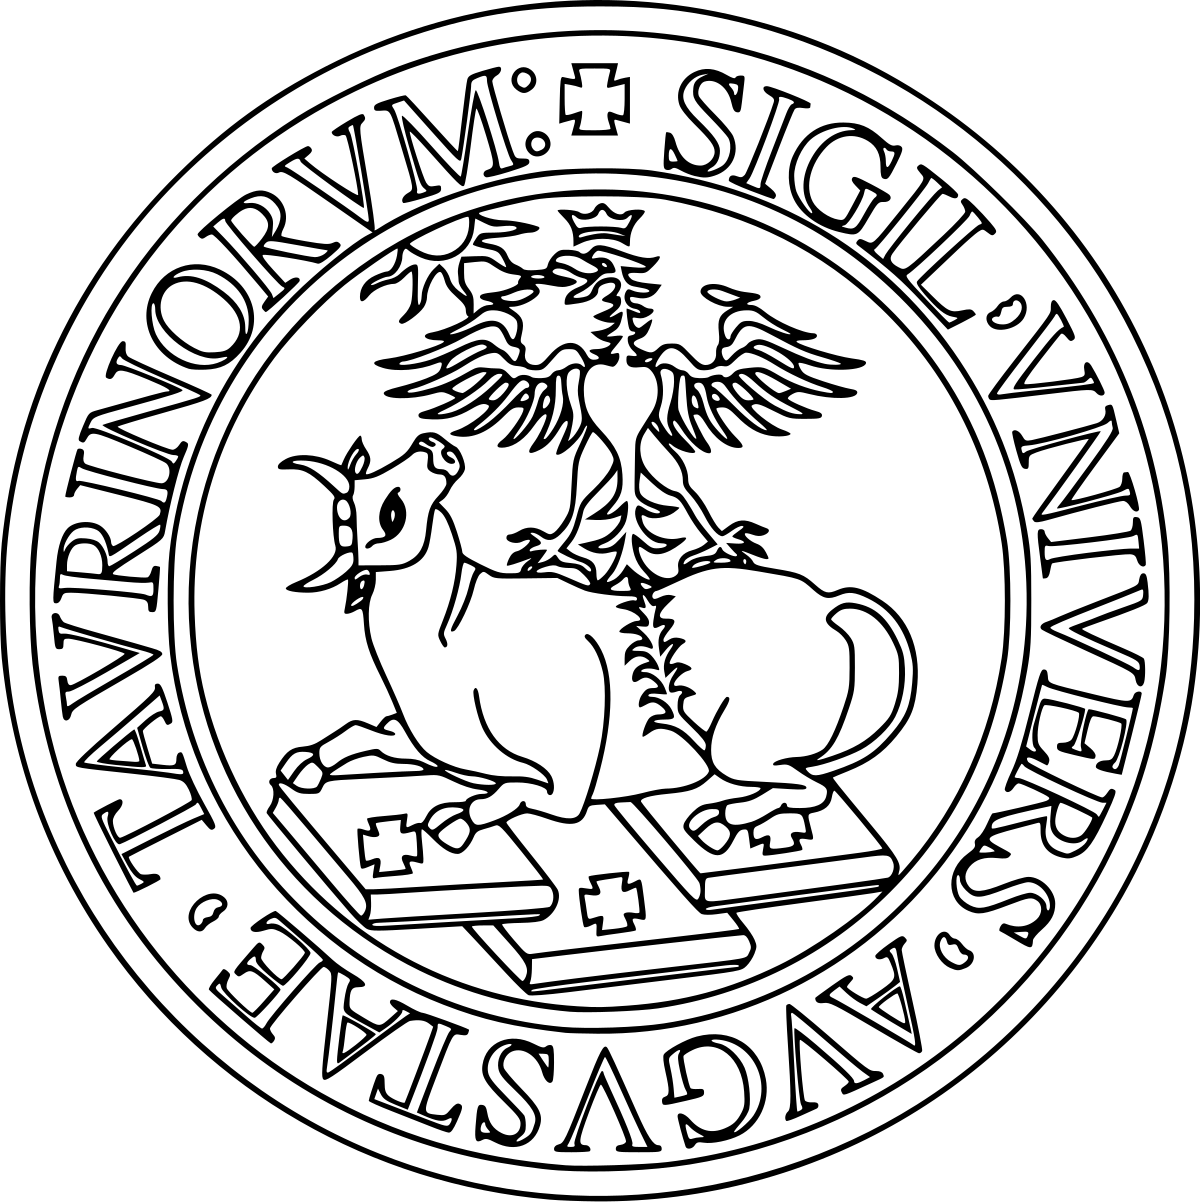
\includegraphics[width=0.2 \textwidth]{Figures/unitologo.png}\\
\vspace{.7cm}
\begin{center}
\LARGE{\textbf{Generative Models as Out-of-equilibrium Particle Systems: the case of Energy-Based Models}}
\end{center}
\vfill
\vspace{.9cm}

\begin{tabular}{l l}
\large Candidate: \hspace{2.5cm} & \large Supervisors: \\
\vspace{1mm}
\Large Davide Carbone \hspace{2.5cm} & \Large Prof. Lamberto Rondoni\\
\hspace{5.5cm} & \Large Prof. Eric Vanden-Eijnden\\
\vspace*{-1cm}
\end{tabular}

\end{center}

\vfill
\vspace{0.7cm}

\begin{center}
XXXVI cycle \\
Academic years 2020-2021 / 2021-2022 / 2022-2023
\end{center}
\end{titlepage}

\frontmatter

\newpage
\mainmatter

\clearpage
\begin{flushright}
    \thispagestyle{empty}
    \vspace*{\fill}
    {\em A Mamma, Papà e Andrea\\}
    \vspace*{\fill}
\end{flushright}
\clearpage

\chapter*{Acknowledgements}
%\subfile{EBM/aknow}
\pagestyle{fancy}
\fancyhf{}
\renewcommand{\chaptermark}[1]{\markboth{\thechapter.\ #1}{}}
\renewcommand{\sectionmark}[1]{\markright{\thesection\ #1}}
\fancyhead[LE,RO]{\thepage}
\fancyhead[CE]{\nouppercase{\leftmark}}
\fancyhead[CO]{\nouppercase{\rightmark}}

%\addcontentsline{toc}{chapter}{Acknowledgements}


\clearpage{\pagestyle{empty}\cleardoublepage}

\chapter*{Abstract}
\addcontentsline{toc}{chapter}{Abstract}
%\subfile{EBM/abstract}




\clearpage{\pagestyle{empty}\cleardoublepage}

\tableofcontents

\clearpage{\pagestyle{empty}\cleardoublepage}

%\listoffigures




%\pagestyle{plain}
\pagestyle{fancy}
\fancyhf{}
\renewcommand{\chaptermark}[1]{\markboth{\thechapter.\ #1}{}}
\renewcommand{\sectionmark}[1]{\markright{\thesection\ #1}}
\fancyhead[LE,RO]{\thepage}
\fancyhead[CE]{}
\fancyhead[CO]{}
\setlength\parindent{0pt}

\newcommand{\R}{\mathbb{R}}
\newcommand{\E}{\mathbb{E}}
\newcommand{\PP}{\mathbb{P}}
\newcommand{\N}{\mathbb{N}}
\newcommand{\Z}{\mathbb{Z}}
\newcommand{\T}{\mathsf{T}}



\clearpage{\pagestyle{empty}\cleardoublepage}


%%%%%%%%%%%%%%%%%%%%%%%%%%%%%%%%%%%%%%%%%%%%%%%%%%%%%%%%%%%%%%

\part{Main Content. Generative Models as Out-of-equilibrium Particle Systems: the case of Energy-Based Models}
\label{blx:refsection\therefsection}
Part of the work described in this section has also been previously published in:
\begin{itemize}
\item D. Carbone, M. Hua, S. Coste, and E. Vanden-Eijnden. \emph{Generative models as out-of-equilibrium particle systems: training of Energy-Based Models using Non-Equilibrium Thermodynamics}. To appear in: Proceedings of the 2nd International Conference on Nonlinear Dynamics and Applications (ICNDA), 2024
\item D. Carbone, M. Hua, S. Coste, and E. Vanden-Eijnden. \emph{Efficient Training of Energy-Based Models
Using Jarzynski Equality}. In: Proceedings of 37th Conference on Neural Information Processing Systems (NeurIPS), 2023
\end{itemize}


%qui metti i file esterni

%\chapter{Introduction}
%\label{blx:refsection\therefsection}
%\subfile{EBM/Introduction}






%%%%%%%%%%%%%%%%%%%%%%%%%%%%%%%%%%%%%%%%%%%%%%%%%%%%%%%%%%%%%%% 

\printbibheading
\bibbysection[heading=bibbysubsect]

	
\end{document}



